%%%%%%%%%%%%%%%%%%%%%%%%%%%%%%%%%%%%%%%%%%%%%%%%%%%%%%%%%%%%%%%
%
% Welcome to Overleaf --- just edit your LaTeX on the left,
% and we'll compile it for you on the right. If you open the
% 'Share' menu, you can invite other users to edit at the same
% time. See www.overleaf.com/learn for more info. Enjoy!
%
%%%%%%%%%%%%%%%%%%%%%%%%%%%%%%%%%%%%%%%%%%%%%%%%%%%%%%%%%%%%%%%

% ===============================================
% MATH 790: Real Analysis           Spring 2022
% hw_template.tex
% ===============================================

% -------------------------------------------------------------------------
% The preamble that follows can be ignored. Go on
% down to the section that says "START HERE" 
% -------------------------------------------------------------------------

\documentclass{article}

\usepackage[margin=1in]{geometry} 
\usepackage{amsmath,amsthm,amssymb,hyperref}
\usepackage{enumitem}
\usepackage{graphicx}
\graphicspath{ {./images/} }

\newcommand{\R}{\mathbf{R}}  
\newcommand{\Z}{\mathbf{Z}}
\newcommand{\N}{\mathbf{N}}
\newcommand{\Q}{\mathbf{Q}}

\newenvironment{theorem}[2][Theorem]{\begin{trivlist}
\item[\hskip \labelsep {\bfseries #1}\hskip \labelsep {\bfseries #2.}]}{\end{trivlist}}
\newenvironment{lemma}[2][Lemma]{\begin{trivlist}
\item[\hskip \labelsep {\bfseries #1}\hskip \labelsep {\bfseries #2.}]}{\end{trivlist}}
\newenvironment{exercise}[2][Exercise]{\begin{trivlist}
\item[\hskip \labelsep {\bfseries #1}\hskip \labelsep {\bfseries #2.}]}{\end{trivlist}}
\newenvironment{problem}[2][Problem]{\begin{trivlist}
\item[\hskip \labelsep {\bfseries #1}\hskip \labelsep {\bfseries #2.}]}{\end{trivlist}}
\newenvironment{question}[2][Question]{\begin{trivlist}
\item[\hskip \labelsep {\bfseries #1}\hskip \labelsep {\bfseries #2.}]}{\end{trivlist}}
\newenvironment{corollary}[2][Corollary]{\begin{trivlist}
\item[\hskip \labelsep {\bfseries #1}\hskip \labelsep {\bfseries #2.}]}{\end{trivlist}}

\newenvironment{solution}{\begin{proof}[Solution]}{\end{proof}}

\begin{document}

% ------------------------------------------ %
%                 START HERE                  %
% ------------------------------------------ %

\title{Problem Set 1} % Replace with appropriate title
\author{Gabriel Casabona\\Physics 332, Statistical Mechanics} % Replace "Author's Name" with your name

\maketitle

% -----------------------------------------------------
% The following two environments (theorem, proof) are
% where you will enter the statement and proof of your
% first problem for this assignment.
%
% In the theorem environment, you can replace the word
% "theorem" in the \begin and \end commands with
% "exercise", "problem", "lemma", etc., depending on
% what you are submitting. 
% -----------------------------------------------------

\begin{problem}{(Nature of temperature)} // 
	\begin{enumerate}[label=\alph*)]
		\item From my understanding, temperature describes the motion of the particles in a given system. Specifically, the way that they vibrate in a given medium. Particles in motion have kinetic energy, by definition, therefore it is reasonable to deduce that energy and temperature are related.
		\item A hot cup of coffee, assuming it is not being intentionally insulated, will cool down to the temperature of the outside system. Technically speaking, the coffee and the atmosphere around it will eventually reach thermal equilibrium. Given the typical scales of coffee and the volume of the space around it, i.e the room, a hot cup of coffee will cool down to room temperature.
		\item Adding energy to a pot of \textit{boiling} water will cause the individual molecules to vibrate faster. It's temperature will change, but it's important to note that since the water is already boiling, it will just turn to gas quicker.
	\end{enumerate}
\end{problem}

\begin{problem}{(Identification of the temperature)} //
	\begin{enumerate}[label=\alph*)]
		\item It takes about 4 seconds for the simulation to reach equilibrium, which I determined by looking for when the kinetic and potential energies stopped fluctuating. The average potential energy for the red particles is -243, and for the green particles is -281.6. The average kinetic energy for the red particles is 7.29. and for the green particles is 9.6. The total energy of each system is constant, which it should be since energy is always conserved.

			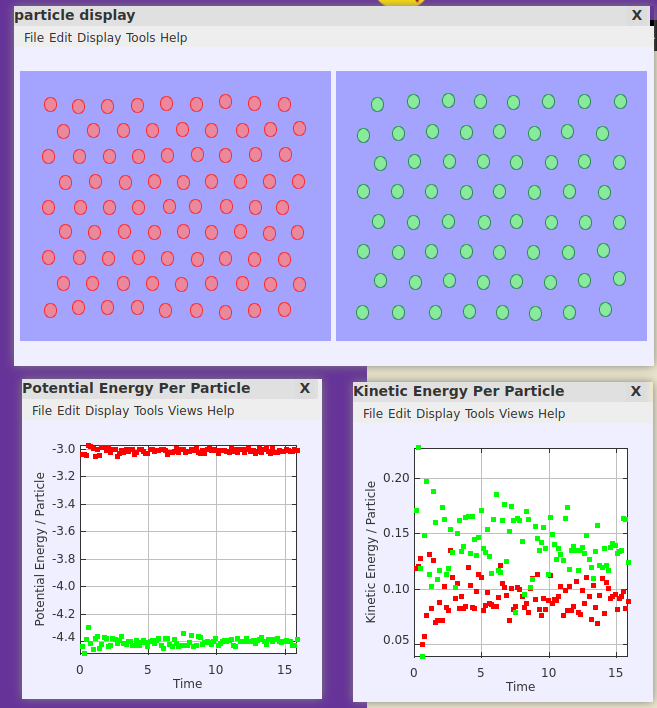
\includegraphics[scale=0.2]{2a.png}

		\item Energy is exchanged between the two systems. This can be shown by the large oscillations of kinetic energy shown in the plot below.
			
			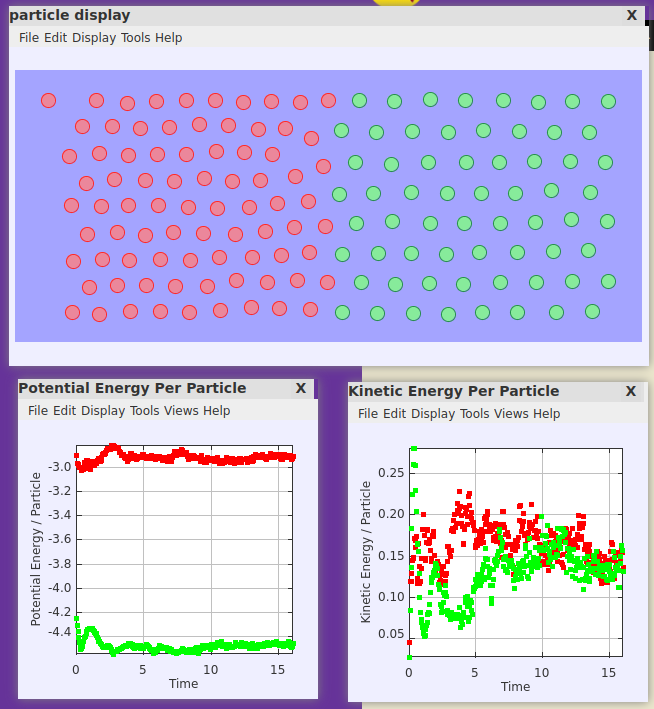
\includegraphics[scale=0.2]{2b.png}

		\item The average potential energy of the systems remained about the same as before the boundary was removed. The kinetic energies are now different, red is about 12.96 and green is 10.24.

			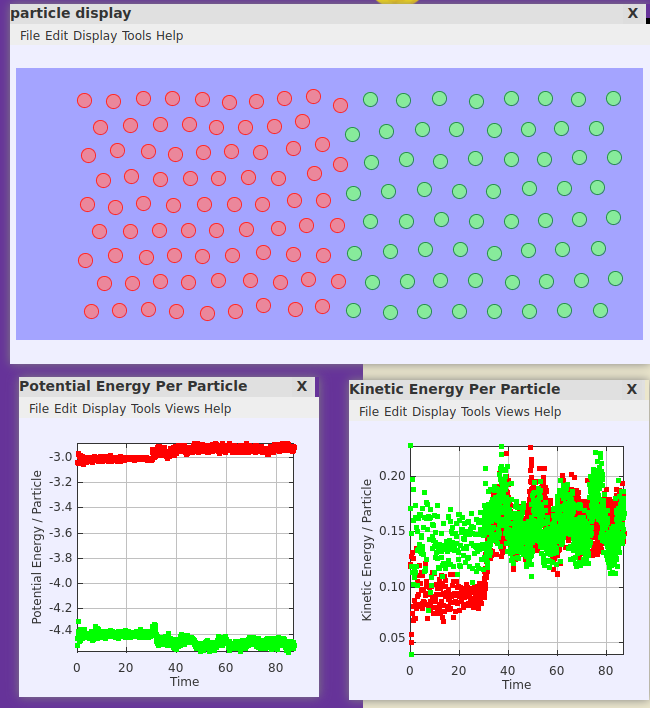
\includegraphics[scale=0.2]{2c.png}

		\item Kinetic energy seems to remain the same for both systems after equilibrium is reached. It makes more sense to compare the average total energies as opposed to per particle, since we are dealing with a large amount of them. The temperature of the system seems to be more closely related to the average kinetic energies.
	\end{enumerate}
\end{problem}


\begin{problem}{(Irreversibility)} //
        \begin{enumerate}[label=\alph*)]
                \item After 60 seconds, the particles remain in a straight vertical line. 

                        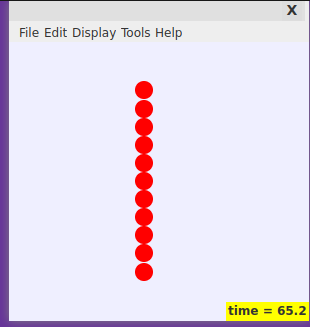
\includegraphics[scale=0.2]{3a.png}

                \item The particles break apart. The system exhibits new behavior in about one second.

                        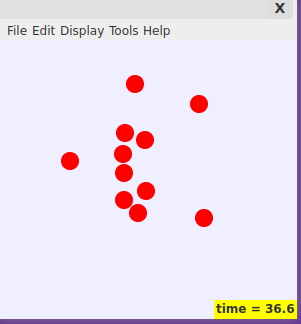
\includegraphics[scale=0.2]{3b.png}

                \item The maximum amount of time allowed for the particles to be able to return back to their initial state is about 22. 

                        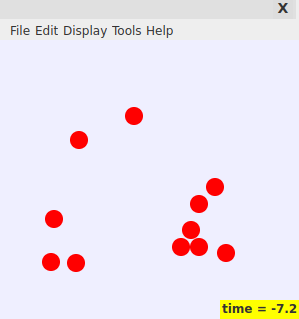
\includegraphics[scale=0.2]{3c.png}

        \end{enumerate}
\end{problem}




% ---------------------------------------------------
% Anything after the \end{document} will be ignored by the typesetting.
% ----------------------------------------------------

\end{document}
